

\documentclass[aspectratio=169, 12pt]{beamer}

%%%%%%%%%%%%
% Packages %
%%%%%%%%%%%%

\usepackage{ctex}
\usepackage[english]{babel}
\usepackage{packages/sleek}
\usepackage{packages/tweaks}
\usepackage{calligra} % thanks pakeage

%%%%%%%%%%%%%%%%
% Bibliography %
%%%%%%%%%%%%%%%%

\addbibresource{./resources/bib/references.bib}

%%%%%%%%%%%%%%
% Title-page %
%%%%%%%%%%%%%%


\title{公共经济学}
\subtitle{Based on Metropolis theme}
\author[LIU ShHUAI]{刘 {  } 帅}
\institute{山西师范大学 {  } 经济与管理学院}
\date{\today}
\titlelogo{./resources/pdf/logo.png}
\framelogo{./resources/pdf/logo.png}

%%%%%%%%%%%%
% Document %
%%%%%%%%%%%%

\begin{document}

\maketitle

\begin{frame}[standout]
    案例分析三\par
    \addtolength{\parskip}{.4em}
    我国高速公路有效供给的困境与对策分析
\end{frame}

\begin{frame}[plain]
    % \begin{multicols}{1}
    %   \frametitle{Outline}
    %   \tableofcontents[hideallsubsections]
    % \end{multicols}
    \frametitle{Outline}
    \tableofcontents[hideallsubsections]
    % \tableofcontents[currentsection]
  \end{frame}

\section{内容提要}

\begin{frame}[plain]
    \frametitle{内容提要}
    2012年9月我国政府开始实施“高速公路节假日免费开放”政策,却引发
了严重的拥堵问题,如何进一步提高高速公路使用效率,实现其科学收费与免
费期间的科学利用成为实现公共产品有效供给的典型问题。本案例首先对不同情境
下高速公路的公共产品属性进行探讨,阐释高速公路的收费原理,分析高速公
路延期收费、收费标准过高问题的根源;其次,运用经济学原理,分析高速公路
免费开放导致严重拥堵的原因,借鉴发达国家与地区高速公路供给的先进经验,
提出实现我国高速公路有效供给的对策建议。
\end{frame}

\section{一、案例导入}

\begin{frame}{plain}
    \frametitle{导入案例}
    2012年中秋节、国庆节前夕,交通运输部下发《关于切实做好重大节假日免
收小型客车通行费有关工作的通知》;截至9月23日,北京、上海、山东等20多
个省份公布了国庆假期收费公路免费的实施细则。大部分省份明确规定,包括机
场高速和桥梁、隧道在内的收费公路免费。2012年11月22日,交通运输部新闻
发言人何建中在北京举行的新闻发布会上表示,春节期间继续实行高速公路小
客车免费通行政策。2013年国家出台《重大节假日免收小型客车通行费实施方
案》,由交通运输部发布。免费通行时间包括春节、清明节、劳动节、国庆节四个重
要节假日。
\end{frame}

\begin{frame}{plain}
    \frametitle{导入案例}
    \begin{figure}
        \centering
        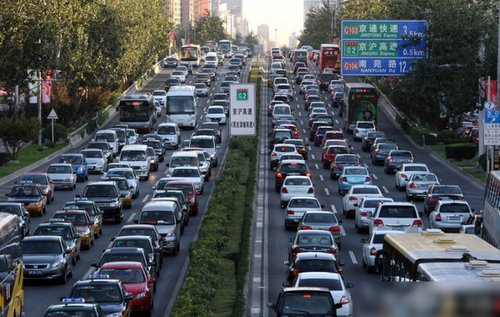
\includegraphics[width=1.0\textwidth]{./resources/figure/trafic.jpg}\
    \end{figure}
\end{frame}

\begin{frame}[plain]
    \frametitle{导入案例}
    2012年10月1日,在上海工作的刘长荣准备趁“双节”假期,回扬州探亲。
“早上6点钟就从上海出发了,11点还没有过苏州。”刘长荣颇为无奈地说。本
以为提前出发可以避开高峰期,可是7点多从上海花桥收费站上高速之后才发
现,车子已经堆积了起来。“因为事故频发,早上已经有好几次堵车了,就算不
堵车,车子也基本低速行驶。晚上8点,刘长荣才到了常州段。期间,刘长荣在
无锡的高速服务区进行了短暂休息。“这个服务区平时从来没有这么繁忙过,现
在连停车位都没有,加油要排队整整40分钟。更令人诧异的是,服务区里的不
少食品和饮料已经销售一空。”刘长荣表示,在这半天时间里,他在高速公路上
就目睹了近10起事故,虽然都是一些追尾的小事故,但却严重影响了车辆的正
常行驶。同年,扬州日报指出该报排名第一的微博热门话题就是“高速路上发微
博”。截至9月30日15时,共生成75039031条关于“高速拥堵”的微博信息,
上演现实版的“人在囧途”。
\end{frame}

\section{二、前言}

\begin{frame}{plain}
    \frametitle{前言}
    高速公路在我国的交通运输中占据重要地位。尽管我国高速公路总里程仅占公路网总里程的2\%左右,但却承担着20\%以上的汽车行驶量,特别是“贷款修路,收费还贷”政策实施以来,高速公路建设摆脱不了国家资金不足的约束,形成了依靠自身滚动发展的良性循环机制,推进了高速公路跨越式发展。
\end{frame}

\begin{frame}{plain}
    \frametitle{前言}
    然而,现行的政府主导、多元化投资、市场化运作的高速公路投资体制,在保证建设资金和效率的同时,又带来了新的问题:高速公路准公共产品属性与企业市场化运营的商品逐利性产生的矛盾;高速公路的社会效益目标和经济效益要求之间的冲突;部分高速公路在收回贷款后,仍然延长收费年限;与其他国家和地区相比,高速公路收费标准偏高等。这些问题的存在,使得公众对高速公路回归公共产品属性的呼声日益高涨。
\end{frame}

\begin{frame}[plain]
    \frametitle{前言}
    高速公路具有公共产品性质,但我国高速公路的建设与发展具有特殊性,单纯依靠政府或市场供给不能达到高速公路供给的有效性,需要通过有偿使用的方式实现其使用价值。多年来,关于我国高速公路有效供给的研究成果有三种倾向性观点:一是高速公路收费的必要性。二是我国高速公路收费存在的问题。三是高速公路有效供给的对策措施。
\end{frame}

\begin{frame}[plain]
    \frametitle{前言}
    这些研究为本章提供了理论借鉴和研究平台,但是由于现有研究较少考虑拥挤对高速公路产品属性的影响,没有限定高速公路收费的条件,且所提对策难以有效解决我国高速公路供给中存在的困境。本案例以我国高速公路有效供给为研究对象,在界定高速公路的公共产品性质的基础上,分别对我国高速公路收费中存在的过期收费与收费过高、免费时引发的道路拥挤等现象进行经济学分析;通过借鉴国际经验,提出确保高速公路有效供给的对策建议。
\end{frame}

\section{三、高速公路的公共产品属性}

\begin{frame}[plain]
    \frametitle{高速公路的公共产品属性}
    公共产品具有与私人产品不同的特征,即消费的非排他性和非竞争性。
    在分析高速公路的产品性质时,引入两个参数。一是竞争性判别参数$\delta $。
    边际拥挤成本由服务或产品的数量$Q$决定,也是高速公路消费竞争性的原因。
    当$Q$大于最小拥挤量时,$\delta =1$,存在竞争性;当$Q$小于最小拥挤量时,$\delta =0$,
    不存在竞争性。二是经营性系数,用以判定高速公路的排他性。
    把高速公路的经营性系数定义为高速公路市场价值$V$与建造成本$C$之比。
    当它们之比$R$为零时,高速公路免费开放,不具有排他性;它们之比$R$越大,
    收益越高,高速公路的排他性也越强。
\end{frame}

\begin{frame}[plain]
    \frametitle{高速公路的公共产品属性}
    (1)$\delta =0,R=0$.此时,高速公路的收费为0,不具有排他性,且行驶车流量较少,不存在竞争性,高速公路属于纯公共产品。
    \par
    (2)$\delta =1,R=0$.此时,高速公路的收费为0,不具有排他性。但是,此时的车流量较大,存在一定的拥挤成本。
    \par
    (3)$\delta =0,R<1$。高速公路不具有竞争性,但需要收取一定的费用,属于准经营性自然垄断产品,行驶车辆不产生拥挤成本。
\end{frame}

\begin{frame}[plain]
    \frametitle{高速公路的公共产品属性}
    (4)$\delta =1,R<1$.高速公路属于准经营性的公共产品,排他性不强,行驶车辆较多,有一定的拥挤成本。
    \par
    (5)$\delta =0,R>=1$.高速公路不存在竞争性,但排他性较高,属于经营性自然垄断产品。
    \par
    (6)$\delta =1,R>=1$.高速公路既具有高竞争性,也具有高排他性,是典型的私人产品。
\end{frame}

\begin{frame}[plain]
    \frametitle{高速公路的公共产品属性}
    对于(1)、(2)两类高速公路,市场投资将难以实现有效供给,政府只能把它们当作公益性投资,成本高昂;对于(3)、(4)类高速公路,它们的经营性系数小于1,表明高速公路定价过程中的收费小于成本,需要政府投资;对于(5)、(6)两类高速公路,它们的收费大于成本,可以通过市场机制供给,由于政府对高速公路收费有着严格的控制,且市场竞争也将导致收费水平下跌,(5)、(6)两类高速公路在我国并不存在。
\end{frame}

\begin{frame}[plain]
    \frametitle{高速公路的公共产品属性}
    依据竞争性参数$\delta $和经营性参数$R$,可以得出以下结论:
    第一,高速公路收费时,$R<1$,是具有一定排他性的准公共产品,且一旦车流量过于拥挤,也具有一定的竞争性。
    第二,高速公路免费时,$R=0$,不具有排他性,且如果车流量较小,$\delta =0$,高速公路也不具有竞争性,是纯公共产品;如果车流量超过高速公路的最小拥挤量,$\delta =1$,又将因拥挤成本的存在而使高速公路具有一定的竞争性,转化为准公共产品。
\end{frame}

\section{四、我国高速公路收费供给的失效分析}

\begin{frame}[plain]
    \frametitle{(一)高速公路收费的合理性}
    高速公路的非竞争性和非排他性是有一定界限的。在拥挤的高速公路上,每增加一辆车通行,都会使拥挤的程度更严重,导致所有通行的车辆速度降低、出行时间延长、个人和社会成本增加,进而迫使一些车辆放弃使用该高速公路。因此,当告诉公路车流量达到饱和状态时,就会破坏它的公共服务性质。
\end{frame}

\begin{frame}[plain]
    \frametitle{(一)高速公路收费的合理性}
    公共产品理论认为对具有一定限度排他性和竞争性的高速公路,收费可以作为降低道路拥挤程度、提高通行效率的手段。假设高速公路的使用只产生正外部性,且排他成本不随车流量和车型的变化而变化。如下图所示:
\end{frame}

\begin{frame}[plain]
    \frametitle{(一)高速公路收费的合理性}
    \begin{figure}
        \centering
            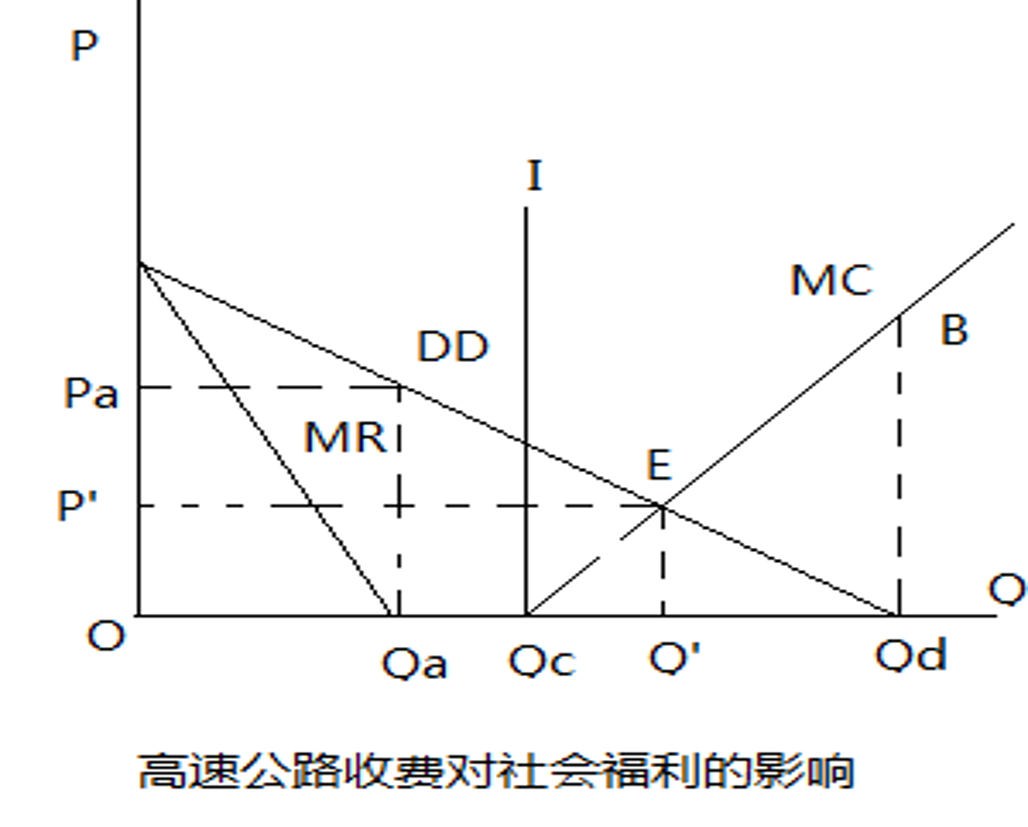
\includegraphics[width=0.75\textwidth]{./resources/figure/charge.png}
        \end{figure}
\end{frame}

\begin{frame}[plain]
    \frametitle{(一)高速公路收费的合理性}
    在上图中,横轴Q表示高速公路上的车流量,纵轴P表示高速公路供给的成本与价格。公众对高速公路的需求曲线为DD。由于高速公路收费水平越低,将会有更多的人愿意行驶在此条高速公路上,因此,曲线DD的斜率为负。MR表示高速公路供给者所获得的边际收益。通行车辆越多,从每辆车上所获得的收益就越少,因此,MR的斜率也为负。
\end{frame}

\begin{frame}[plain]
    \frametitle{(一)高速公路收费的合理性}
    假设高速公路是由政府提供的,供给量为I,此时能满足的通行量为Qc,那么OQc即为提供高速公路的边际成本MC。在不发生拥挤的情况下,每增加一辆车产生的成本很小,维护费用几乎为零;但是,当通行量超过Qc后,就会产生拥挤现象,通行量超过了高速公路的负担能力,MC开始从零上扬。如果在通行量超过Qc后仍然免费供给高速公路,必然会产生拥挤现象,降低同行者的效用,直至通行量达到Qd。此时,Qd与MC交点B是在高速公路免费开放条件下供给者付出的边际成本,三角形EBQd是由消费者获得的效用不足以补偿其消费成本而引起的社会福利净损失。
\end{frame}

\begin{frame}[plain]
    \frametitle{(一)高速公路收费的合理性}
    为了避免由高速公路过度消费引起的社会福利净损失,在高速公路供给量无法在短时间内增加的前提下,可以采取收费的方法提高高速公路的供给效率。按照社会福利最大化标准,收费水平为MC与DD的交点E所决定的价格P’。而高速公路一旦恢复收费,通行量就会从免费时期的Qd减少到Q’,此时将有Qd-Q’的客流量分离而去。
\end{frame}

\begin{frame}[plain]
    \frametitle{(一)高速公路收费的合理性}
    高速公路的公共产品属性并不意味着一定要由公共部门来免费供给。在上图中的分析结果表明,在高速公路通行量达到一定规模时,采用收费的手段能够保证高速公路使用效率的和功能的正常发挥;如果仍然采用免费供给的模式,将导致个人边际效用和社会边际效用低于提供高速公路供给的边际成本,进而带来社会福利的净损失。因此,高速公路收费具有一定的合理性。
\end{frame}

\begin{frame}[plain]
    \frametitle{(二)高速公路收费引发的效率损失}
    制定高速公路的收费水平是一个复杂的过程,既与高速公路供给与需求相关,又与高速公路供给者的经济效益、消费者的经济效益和社会福利相关。特别是高速公路中所包含的经营性高速公路,具备自然垄断的条件,由市场机制来决定高速公路的收费水平必然造成一定的效率损失。如下图所示:
\end{frame}

\begin{frame}[plain]
    \frametitle{(二)高速公路收费引发的效率损失}
    \begin{figure}
        \centering
            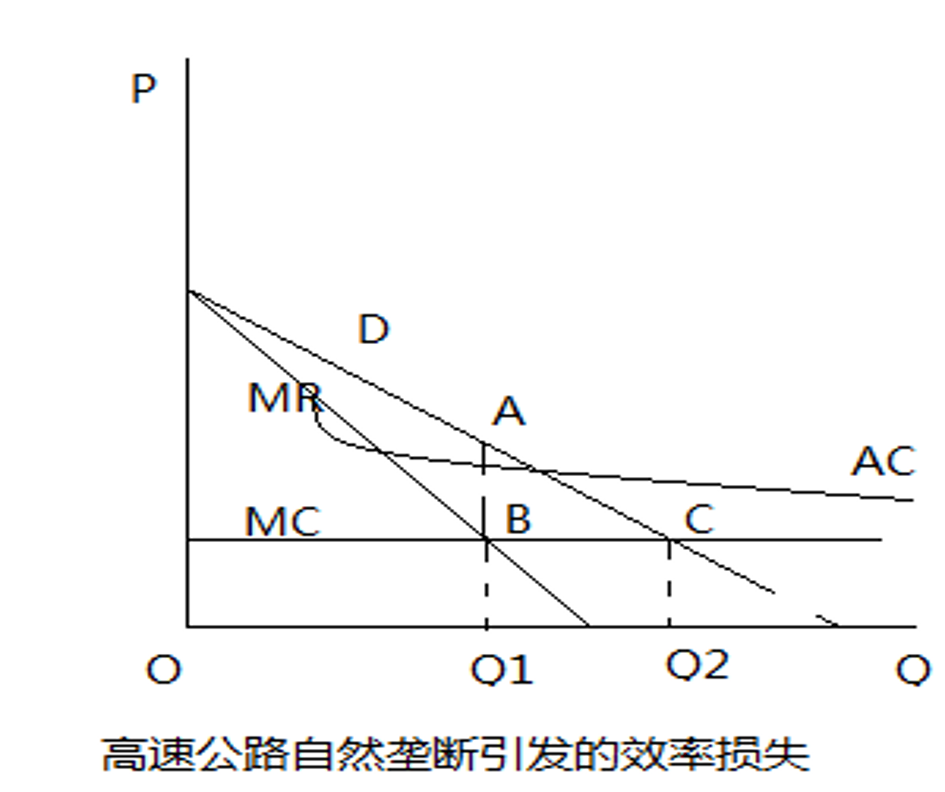
\includegraphics[width=0.7\textwidth]{./resources/figure/loss.png}
        \end{figure}
\end{frame}

\begin{frame}[plain]
    \frametitle{(二)高速公路收费引发的效率损失}
    在上图中,纵轴表示高速公路的收费水平P,横轴表示高速公路供给量Q。由于高速公路具有自然垄断性,因此它的供给成本随供给量的增长而递减,即平均成本曲线AC向右下方倾斜。作为准公共产品的高速公路的需求曲线D在边际收益曲线MR的右侧,边际成本曲线MC是一条无弹性平行于横轴的直线。由边际成本曲线MC和需求曲线D的交点决定的供给量Q2符合社会福利最大化原则。但是在市场机制作用下,高速公路的垄断者会把供给量确定在边际成本曲线MC和边际收益曲线MR的交点B处,高速公路供给量缩减至Q1.此时,若消费者想获得Q2的供给量,只能提高价格,由此造成了数量为三角形ABC面积的效率损失。
\end{frame}

\begin{frame}[plain]
    \frametitle{(三)高速公路收费导致的寻租现象}
    对具有自然垄断特征的行业,在市场竞争机制无法有效供给的前提下,只能通过政府干预提高供给效率。政府干预高速公路的手段主要有:限制高速公路经营者数量,避免市场竞争造成的效率损失;通过收费水平管制规制高速公路经营者的垄断利润;通过服务范围和质量控制避免垄断经营造成的服务水平下降。
\end{frame}

\begin{frame}[plain]
    \frametitle{(三)高速公路收费导致的寻租现象}
    政府对高速公路的收费水平管制是一种经济性调节政策,目的是使高速公路资源配置趋向与帕累托最优。但是,在高速公路收费过程中,与收费水平相关的财务信息不公开,导致高速公路供给者和消费者之间信息的不对称;高速公路的投融资体制以及供给的公平性也存在一定的缺陷;特别是部分与高速公路供给相关部门将部门利益最大化作为行政目标而进行局部逐利,进而导致部门或个人的寻租、设租行为。
\end{frame}

\begin{frame}[plain]
    \frametitle{(三)高速公路收费导致的寻租现象}
    按照公共选择理论,高速公路“寻租-涉租”关系源于政府对高速公路市场的干预。政府干预不是一定会导致寻租活动,但却为寻租活动创造了条件。寻租、涉租行为带来的效率损失表现在:寻租者花费时间、精力和金钱去游说或疏通关系,提升了自己的效率却降低了社会效率;寻租活动会导致政府部门之间及官员之间争权夺利,妨碍公共决策的执行,降低行政效率。高速公路收费中的寻租、设租行为使得收费额度与社会边际成本、个人边际成本相关外,还要再加上寻租、设租的社会成本,进而导致高速公路收费水平的无限度上升或厌其收费问题。
\end{frame}

\section{五、我国高速公路免费通行的拥挤分析}

\begin{frame}[plain]
    \frametitle{(一)高速公路免费供给带来产量不足}
    \begin{figure}[]
        \centering
        \begin{minipage}{0.4\linewidth}
            高速公路免费供给的效率表现在政府是否提供了充足的免费高速公路,提供的数量是否能够满足消费者的需要。如右图所示:
        \end{minipage}%
        \begin{minipage}{0.6\linewidth}
            \centering
            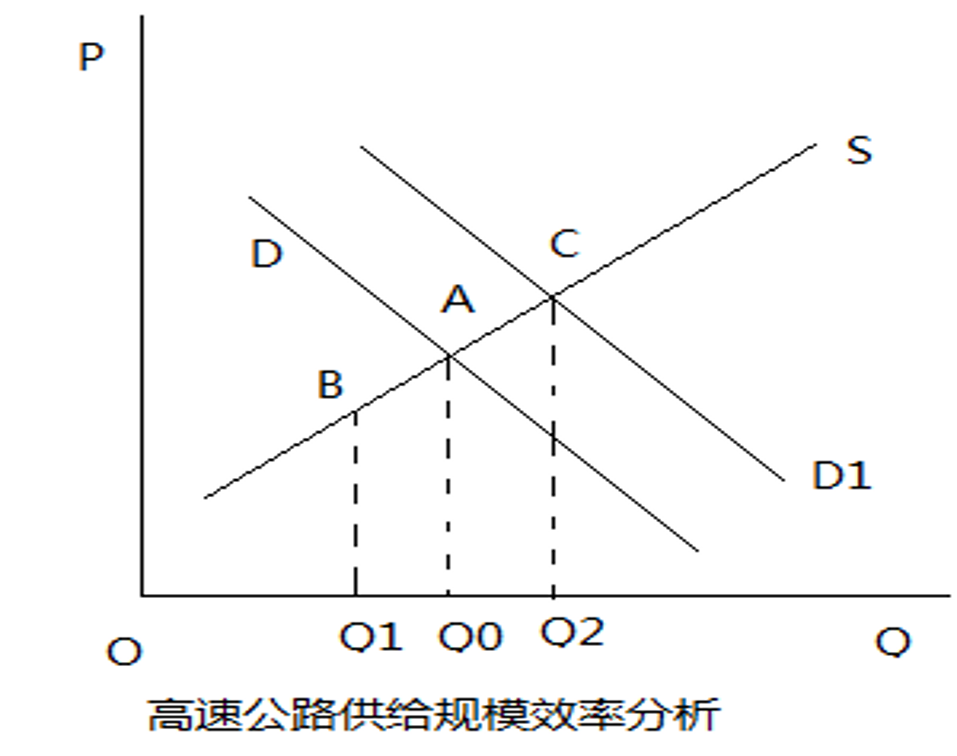
\includegraphics[width=1.0\textwidth]{./resources/figure/supply.png}
        \end{minipage}
        \end{figure}
\end{frame}

\begin{frame}[plain]
    \frametitle{(一)高速公路免费供给带来产量不足}
    在上图中纵轴表示高速公路收费水平,横轴表示消费者的供给需求量。曲线D代表高速公路需求曲线,曲线S代表高速公路供给曲线,二者在均衡条件下相交于A点。A点所对应的高速公路供给需求量Q0是政府能够供给且使用者愿意接受的产量。
\end{frame}

\begin{frame}[plain]
    \frametitle{(一)高速公路免费供给带来产量不足}
    事实上,免费高速公路是有限的,其均衡量不能达到Q0,供给曲线S上的供给量下降至B点所对应的产量为Q1,但免费高速公路的诞生将改变消费者的需求,需求曲线转变为一条平行于D且高于D的曲线D1,与供给曲线S相交于C,且对应的需求量为Q2。显然消费者的需求量与供给量存在Q2-Q1的差值,是产量不足无法弥补的。尽管如此,消费者不会因为供给不足而放弃消费;反之,正因为高速公路免费带来的非排他性而纷纷拥挤到同一条公路上来,造成高速公路拥挤严重。
\end{frame}

\begin{frame}[plain]
    \frametitle{(二)高速公路免费供给造成过度消费}
    \begin{figure}[]
        \centering
        \begin{minipage}{0.4\linewidth}
            在免费供给时,高速公路转化为同时具有非排他性、非竞争性和稀缺性的纯公共产品。稀缺性公共产品容易产生“搭便车”现象,带来的结果是对该公共产品的实际消费量超过预期消费量,即过度消费。高度消费增加到一定程度,就是拥挤问题。如右图所示:
        \end{minipage}%
        \begin{minipage}{0.6\linewidth}
            \centering
            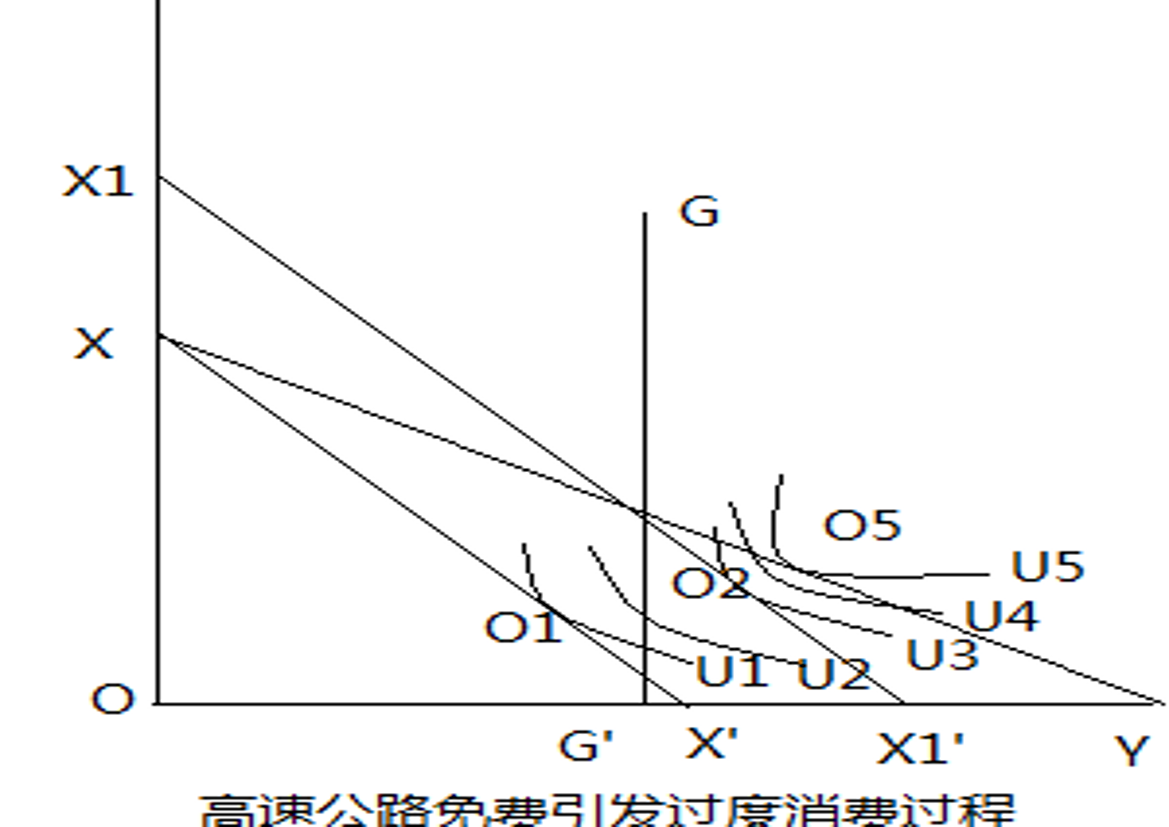
\includegraphics[width=1.0\textwidth]{./resources/figure/consum.png}
        \end{minipage}
        \end{figure}
\end{frame}

\begin{frame}[plain]
    \frametitle{(二)高速公路免费供给造成过度消费}
    假设驾车出行者全部为理性“经济人”,他们在选择如何消费的过程中,总是在预算线约束下,使用最少的成本以获取最大收益。在上图中,横轴为行驶车辆数,纵轴为驾车出行者的效用,XX’为高速公路收费期间的驾车出行者预算线,GG’为高速公路的供给量。此时驾车出行者可以达到的最大效用为U1,效用曲线U1与预算线相切与O1点,即驾车出行者选择的高速公路需求量小于高速公路的供给量。
\end{frame}

\begin{frame}[plain]
    \frametitle{(二)高速公路免费供给造成过度消费}
    在高速公路免费开放期间,因收费价格发生相对变化,预算线斜率发生变动,预算线XX’移到XY。当高速公路供给充足时,驾车出行者的无差异曲线U5同新的预算线XY相切与Q5点,即驾车出行者在Q5点达到效用最大化。但是高速公路的供给量是有限的,依然是GG’,Q5点并不能真正出现。但是,在追求Q5点的动机作用下,驾车出行者的需求大于高速公路的供给量,造成道路拥挤和交通事故。结果是在高速公路免费开放的条件下,驾车出行者对高速公路的需求量与高速公路供给量之间的差额为Y-G’。
\end{frame}

\begin{frame}[plain]
    \frametitle{(三)高速公路免费供给引发搭便车行为}
    搭便车是指不付成本而坐享其成他人之利的投机行为。公共产品的非排他性和非竞争性为产品的供给和消费搭便车提供了空间。搭便车行为导致“公地悲剧”:人们会最大限度地利用公共资源并以牺牲公共利益为代价追求个人利益。
\end{frame}

\begin{frame}[plain]
    \frametitle{(三)高速公路免费供给引发搭便车行为}
    高速公路免费供给为搭便车行为提供了条件,进而导致高速公路通行量突破最小拥堵通行量。为了便于分析,我们设A为消费者可以选择的高速公路集合,c为收费公路集合,f为免费公路集合;高速公路总里程为L,免费里程为m;高速公路饱和承载人数为N。当只存在收费高速公路时,A=\{c\},部分高速公路免费开放后,A=\{c,f\}。再设市场中存在A型和B型高速公路消费者,高速公路消费者量U为A型、B型消费者人数之和。其中,对于A型消费者,只要高速公路收费水平在
    他们的心理预期之内,他们会作出使用高速公路的决策;对于B型消费者,除了收费水平之外,他们还要充分了解并在对高速公路的服务质量、拥挤情况、便利程度等感觉满意时,才会转化为A型消费者。此时,当高速公路全部收费时,承载量G(0)=N/L,即为高速公路最小拥堵通行量。
\end{frame}

\begin{frame}[plain]
    \frametitle{(三)高速公路免费供给引发搭便车行为}
    消费者搭便车是人们的非真实需求。这种非真实需求的源头是人们对货币或资源的占有心理。如果一个人在公共产品消费中享受“搭便车”,他便会节省更多的私人货币和资源以增加私人产品的消费,从而达到自己的最大满足。在免费高速公路使用中,处于对免费使用资源的占有心理的“个体”都不愿放弃对这种使用公共资源的搭便车机会,纷纷涌向免费高速公路,导致高速公路拥挤,无法实现帕累托最优状态。
\end{frame}

\section{六、我国高速公路有效供给的对策}

\begin{frame}[plain]
    \frametitle{(一)国外经验}
    西方国家高速公路建设大多经历了一个由政府单独投资到混合性融资,再到政府与企业联合供给、共同建设的过程。在此期间,西方国家纷纷建立起高速公路特许经营制度,并成为高速公路建设和运营的基本形式,为高速公路建设提供了可靠的资金保障。通过特许经营制度建设的高速公路普遍具有收费年限长但收费标准低的特点。
\end{frame}

\begin{frame}[plain]
    \frametitle{(一)国外经验}
    差异化免费政策是指免费开放政策并非“全部免费”而是针对部分路段、部分型号车辆、部分时间实施免费。我国台湾地区以疏通交通为目标采取的差异化免费政策更具有借鉴意义。以2013年春节为例,台湾地区高速公路暂停收费时段为0点至7点,这样可以利用高速公路需求较低的时间段,通过免费来吸引部分需求。同时台湾地区免费对象并非小客车,而是大型运输车辆,以鼓励拼车以及使用公共交通,提高公路实际承载能力。
\end{frame}

\begin{frame}[plain]
    \frametitle{(一)国外经验}
    德国大部分高速公路的维修保养费由政府从税收中支付。表面上德国的小型客车不需单独缴纳高速公路费;但从税收角度看,它们在汽油和柴油价格中以能源税、增值税等形式交给联邦政府,这些税收可以用于高速公路维护和环境保护等。美国大部分高速公路路段实行免费或低收费措施的主要原因是修建高速公路的资金主要来自于税收,实际上,在美国高速公路行驶的车辆已经通过税收先期预付了公路的建设费用。
\end{frame}

\begin{frame}[plain]
    \frametitle{(一)国外经验}
    为了确保高速公路的高速通行,在美国纽约以及周边多个州人们普遍使用电子缴费装置,车主在行驶时将其放在挡风玻璃处,收费站的读码器就会自动对其条形码进行扫描,之后从驾驶者的网上账户中扣去相应的行车费。日本在缓解高速公路拥堵时启用电子收费系统ETC。装在车上的车载器和收费站的天线进行无线通信,汽车以20KM/h以下的速度顺利通过收费站,费用则通过信用卡后期支付。
\end{frame}

\begin{frame}[plain]
    \frametitle{(二)对策措施}
    缓解因收费带来的高速公路拥堵问题应以全体使用者的净收益最大化为目标。首先在制度层面允许各地自行决定免费时段,交通运输部只需要制定规范性的指导意见。各地按照交通运输部指定的指导意见,根据本地区高速公路的通行情况,调整免费路段和时段,以此协调高速公路和普通公路的通行量。其次,高速公路免费车型应以承担较多旅客出行的大客车为主。最后,在政府部分与收费公路经营企业的特许经营协议中,增加对车辆免费通行的范围予以扩大化的约定。
\end{frame}

\begin{frame}[plain]
    \frametitle{(二)对策措施}
    高速公路经营方和政府应当建立完善的高速公路免费通行时段管理体系,具体包括:(1)建立智能交通管理系统,监视和监测高速公路通行情况,并适时发布高速公路通行信息,减少高速公路免费时段常发性拥挤的影响和发生频率。(2)成立高速公路应急管理工作指挥部,对发生的交通秩序混乱情况和交通拥堵迹象立即发出指令,调配警力及时处置,定点、定时、定则管控。(3)加强高速公路大货车免费期间的管理,即对大货车开通专项通道,避免与中小型车辆同时进出造成收费、通行障碍。(4)建立多元利益
    需求表达机制,鼓励公众参与管理。(5)实施目标管理,提高管理水平与服务效率。(6)及时公布高速公路通行信息。
\end{frame}

\begin{frame}[plain]
    \frametitle{(二)对策措施}
    (1)进快制定吸引民间资本进入基础设施建设领域的政策法规,解决目前普遍存在的政策不完善、不配套、不落实的问题。(2)对经济发展具有重要作用的公路项目为吸引民间资本给投资该公路建设项目的民间资本创造合适的利润空间,政府可以采取免税、赠与土地和财政补贴等方式来提高投资者参与意愿。(3)消除对民间投资所有制的歧视,把吸引民间资本的数量作为高速公路相关管理部门政绩考核的重要内容。(4)灵活运用各种融资方式,发挥各自的优势,吸引各层次的民间资本、以不同的形式进入公路建设领域。
\end{frame}

\begin{frame}[plain]
    \frametitle{(二)对策措施}
    根据国外交通发展的实践经验,利用立法形式建立交通设施建设的特定财源制度,可以保证交通设施建设拥有稳定的资金来源。
    \par
    交通设施建设的特定财源主要是指专项基金,其构成是成品油消费税、车辆购置税。在基金建设初期,征收一些高速公路使用费是合理的,随着以税代费政策及证券市场的完善,可以逐步减少高速公路使用费,最终实现高速公路的零收费。
\end{frame}

% ---------------------------------------------------------------------------
\begin{frame}[standout]
    \begin{center}
        {\Huge\calligra Thanks!}
      \end{center}
\end{frame}
% ---------------------------------------------------------------------------

\end{document}
